\chapter{Results and interpretation\label{sec:results}}

\section{Systematic uncertainties\label{sec:results-systematics}}

The following is a list of the sources of systematic uncertainty used in the calculation of the total uncertainty in this search, some of which have been described in previous sections. In the limit calculation, these systematics are all treated as nuisance parameters affecting only the scale of the expected signal or background yields, and they are modelled with log-normal distributions.
%A comprehensive list of uncertainties can be found in Appendix~\ref{sec:errors}.

\begin{itemize}
\item \textbf{Luminosity: } As assessed in summer 2013~\cite{CMS-PAS-LUM-13-001}, the uncertainty on the integrated luminosity is taken to be 2.6\%.
\item \textbf{Muon trigger efficiency: } According to the CMS MUO POG~\cite{CMS:muonuncertaintytwiki}, the systematic uncertainty from the single-muon trigger \texttt{HLT\_IsoMu24\_eta2p1} is 0.2\% for the WH and ZH signals. For the ggH and VBF signals, because of the effect of the nearby lepton filter applied to the trigger muon, a larger systematic uncertainty of 4.2\% is applied (see Sec.~\ref{lepideff-HLT} for details).
\item \textbf{Tight muon ID efficiency: } According to the CMS MUO POG~\cite{CMS:muonuncertaintytwiki}, the systematic uncertainty on the trigger muon tight ID is 0.5\%.
\item \textbf{Muon isolation efficiency: } According to the CMS MUO POG~\cite{CMS:muonuncertaintytwiki}, the systematic uncertainty on the trigger muon isolation is 0.2\%. This is applied to signal events in the WH and ZH channels. For the ggH and VBF channels, an uncertainty of 10\% is used instead, to account for the fact that the muon which fires the trigger comes from a boosted $\tau_{\mu}\tau_{\text{had}}$ topology, and that the isolation efficiency for the trigger muon is largely recovered if the nearby reconstructed tau is subtracted from its isolation cone; the 10\% figure is taken from the Tau POG recommendation for the HPS tau ID efficiency for this boosted configuration.
\item \textbf{Soft muon ID efficiency: } According to the CMS MUO POG~\cite{CMS:muonuncertaintytwiki}, the systematic uncertainty on the $\tau_{\mu}$ ID is 1.5\%.
\item \textbf{HPS ID efficiency: } The accepted value of 6\% from the CMS TAU POG is used~\cite{CMS:tauuncertaintytwiki}.
\item \textbf{Tau charge misidentification rate: } The accepted value of -1\%/+2\% from the CMS TAU POG is used~\cite{CMS:tauuncertaintytwiki}.
\item \textbf{b-veto efficiency: } Two systematic uncertainties are considered for the b-veto efficiency. The first uncertainty stems from the fact that b-veto data/MC scale factors for light jets are applied to the tau jets on which the b-veto is applied; since the actual data/MC scale factors are expected to be somewhere between light jets and b-jets, the percent difference in signal yields when using light jet scale factors and when using b-jet scale factors is taken as a systematic uncertainty, and the magnitude ranges between 1.8-8.5\% depending on the $M_{T}$ bin and signal process. The second source of systematic uncertainty comes from the uncertainty on the light-jet scale factors used; following the BTV recommendations, the scale factors are shifted coherently by $\pm$1$\sigma$, and the difference between the nominal and shifted expected signal yields is taken as the systematic uncertainty; errors range up to 5.2\% depending on signal sample. Because the VBF signal is expected to have a similar selection efficiency as the ggH channel, the errors calculated for each mass point in the ggH channel are applied to the VBF prediction for each analogous mass point; for similar reasons, the errors calculated for the WH channel are applied to the ZH channel.
\item \textbf{ID efficiencies for nearby lepton filter around trigger muon: } Systematics are assigned to the ID efficiency data/MC scale factors of the PF electrons, muons, and taus used for the neighbouring lepton veto around the trigger muon. For the PF electrons, since no ID is applied beyond the requirement that they pass PF reconstruction, have $p_T >$ 7 GeV, and $\abs{\eta} <$ 2.5, we apply a conservative error of 1.1\%, based on the highest uncertainty for the low-$p_T$ electrons passing Loose ID requirements~\cite{CMS:egammauncertaintytwiki}. For the PF muons, since the same soft ID is used as for the reconstructed $\tau_{\mu}$, the same systematics uncertainty of 1.5\% is applied~\cite{CMS:muonuncertaintytwiki}. For the PF taus, a conservative uncertainty of 10\% is used. This came from the suggestion of the CMS TAU POG for the ID efficiency of HPS taus reconstructed from jets via the jet-cleaning method (cf. Section~\ref{sec:evtsel-tauID}) with $p_T >$ 10 GeV; this value was estimated by taking the accepted uncertainty of 6\% from the TAU POG~\cite{CMS:tauuncertaintytwiki}, adding in quadrature the discrepancy of at least 1\% observed between the HPS tau ID efficiencies for our signal and Drell-Yan MC events in the studies described in Chapter~\ref{sec:lepideff}, and rounding upwards.
\item \textbf{Background: } To obtain the final jet-faking-tau background prediction in the $m_{\mu+\text{had}}$ $>$ 4 GeV bin in Region A, we take the unweighted average of the nominal background prediction from Region B and the predictions from the alternative non-QCD (from MC) or all-QCD (from region D data) background shapes. For the systematic uncertainty on this background prediction, we look at the central value $+$($-$)1$\sigma$ of the alternative background shapes and compare it to the final background prediction; the greatest positive (negative) difference between the final background prediction and one of these values is then taken to be the positive (negative) systematic error on the final background prediction. This results in asymmetric systematic errors of +77.6\%/-85.0\% for the low-$M_{T}$ bin and +60.9\%/-59.2\% for the high-$M_{T}$ bin.
\item \textbf{$M_{\text{T}}$: } Following the JME recommendations, errors range up to 12.2\% depending on signal sample. Just as for the b-veto errors, the MET errors calculated for each mass point in the ggH channel are applied to the VBF prediction for each analogous mass point, while the errors calculated for the WH channel are applied to the ZH channel.
\item \textbf{VBF and ZH predictions: } The expected signal yields from the VBF and ZH channels were calculated by scaling the ggH and WH expected yields (from MC) respectively to the appropriate SM cross-sections. To account for the extra element of uncertainty introduced by this indirect method of estimation, the percent difference between the number of VBF (or ZH) events from MC and from the indirect estimation method after the full selection at the 9 GeV pseudoscalar mass point (the only mass point for which MC samples were generated for the VBF and ZH channels) was taken as an estimate of the error on the VBF and ZH predictions for all pseudoscalar mass points. For the low-$M_{T}$ bin, the errors were 23.2\% for VBF and 19.1\% for ZH; for the high-$M_{T}$ bin, the errors were 25.3\% for VBF and 24.3\% for ZH.
\end{itemize}

\section{Observed and expected results\label{sec:results-obsexp}}

Table~\ref{tab:results} shows the expected numbers of signal events from each generated pseudoscalar mass point in each of the $M_{\text{T}}$ bins, followed by the background prediction (obtained from Region B) and the actual number of events observed in Region A for $m_{\mu+\text{had}}$ $>$ 4 GeV.

\begin{table*}[htbh]
\begin{center}
\caption{Observed data, estimated background, and expected signal from each generated pseudoscalar mass point in each of the $M_{\text{T}}$ bins assuming SM cross sections and 100\% Br($H\rightarrow$$aa$$\rightarrow4\tau$)  Only statistical error is shown for the signal, while the full error is shown for the background.\label{tab:results}}
\singlespacing
\begin{tabular}{|c|c|c|c|}
\hline
\multicolumn{2}{|c|}{} & $M_{\text{T}} \le$ 50 GeV & $M_{\text{T}} >$ 50 GeV \\
\hline
\multirow{5}{*}{WH} & $m_{a}$ = 5 GeV & 0.11 $\pm$ 0.05 & 0.10 $\pm$ 0.04 \\
& $m_{a}$ = 7 GeV & 1.5 $\pm$ 0.2 & 3.8 $\pm$ 0.3 \\
& $m_{a}$ = 9 GeV & 2.7 $\pm$ 0.2 & 7.0 $\pm$ 0.3 \\
& $m_{a}$ = 11 GeV & 4.2 $\pm$ 0.3 & 8.8 $\pm$ 0.4 \\
& $m_{a}$ = 13 GeV & 3.5 $\pm$ 0.2 & 9.9 $\pm$ 0.4 \\
& $m_{a}$ = 15 GeV & 3.6 $\pm$ 0.2 & 8.4 $\pm$ 0.4 \\
\hline
\multirow{5}{*}{ggH} & $m_{a}$ = 5 GeV & 0.31 $\pm$ 0.22 & 0 \\
& $m_{a}$ = 7 GeV & 21 $\pm$ 2 & 1.9 $\pm$ 0.6 \\
& $m_{a}$ = 9 GeV & 46 $\pm$ 3 & 7.6 $\pm$ 1.1 \\
& $m_{a}$ = 11 GeV & 64 $\pm$ 3 & 11 $\pm$ 1 \\
& $m_{a}$ = 13 GeV & 63 $\pm$ 3 & 18 $\pm$ 2 \\
& $m_{a}$ = 15 GeV & 41 $\pm$ 3 & 11 $\pm$ 1 \\
\hline
\multirow{5}{*}{ZH} & $m_{a}$ = 5 GeV & 0.03 $\pm$ 0.01 & 0.03 $\pm$ 0.01 \\
& $m_{a}$ = 7 GeV & 0.38 $\pm$ 0.04 & 1.0 $\pm$ 0.1 \\
& $m_{a}$ = 9 GeV & 0.68 $\pm$ 0.05 & 1.9 $\pm$ 0.1 \\
& $m_{a}$ = 11 GeV & 1.1 $\pm$ 0.05 & 2.3 $\pm$ 0.1 \\
& $m_{a}$ = 13 GeV & 0.88 $\pm$ 0.06 & 2.7 $\pm$ 0.1 \\
& $m_{a}$ = 15 GeV & 0.91 $\pm$ 0.06 & 2.3 $\pm$ 0.1 \\
\hline
\multirow{5}{*}{VBF} & $m_{a}$ = 5 GeV & 0.03 $\pm$ 0.02 & 0 \\
& $m_{a}$ = 7 GeV & 2.3 $\pm$ 0.2 & 0.22 $\pm$ 0.06 \\
& $m_{a}$ = 9 GeV & 5.1 $\pm$ 0.3 & 0.9 $\pm$ 0.1 \\
& $m_{a}$ = 11 GeV & 7.0 $\pm$ 0.4 & 1.2 $\pm$ 0.1 \\
& $m_{a}$ = 13 GeV & 6.9 $\pm$ 0.4 & 2.0 $\pm$ 0.2 \\
& $m_{a}$ = 15 GeV & 4.5 $\pm$ 0.3 & 1.3 $\pm$ 0.2 \\
\hline
\multicolumn{2}{|c|}{SM Background} & \begin{tabular}[c]{@{}l@{}}5.41 $\pm$ 1 \stat \\$^{+4.2}_{-4.6}$ \syst\end{tabular} & \begin{tabular}[c]{@{}l@{}}6.08 $\pm$ 1.6 \stat \\$^{+3.7}_{-3.6}$ \syst\end{tabular} \\
\multicolumn{2}{|c|}{Data (observed)} & 7 & 14 \\
\hline
\end{tabular}
\end{center}
\end{table*}

\section{Interpretation\label{sec:results-interpretation}}

\subsection{CLs limit calculation\label{sec:results-limitcalc}}

At the end of the selection sequence, when the final $m_{\mu+\text{had}}$ background prediction (obtained as described in Sec.~\ref{sec:bkgs-jet-fake-unc}) has been normalized according to Sec.~\ref{sec:evtsel-search}, the number of events passing $m_{\mu+\text{had}} >$ 4 GeV are counted. This integral serves as the predicted number of events from background only. The integral of the region A data $m_{\mu+\text{had}}$ distribution above 4 GeV is then compared to the prediction derived from region B. In the context of this search, a significant excess in the region A data would be interpreted as coming from the 2HDM signal.  Assuming no excess, limits are set on the cross section times branching ratio for SM Higgs production and decay to lighter Higgses, which subsequently decay to taus.

Methods from the \texttt{HiggsAnalysis/CombinedLimit} package (full code found at~\cite{CombinedGitHub}, documented in~\cite{CombinedTwiki}) are used to evaluate expected and observed limits in this search. The signal strengths calculated by  are defined as:

\begin{equation}
r_{\text{prod}} = \frac{\sigma_{\text{prod}}\cdot B(H\rightarrow aa \rightarrow4\tau)}{(\sigma_{\text{prod}})_{\text{expected}}} \\
\label{eq:rDefinition}
\end{equation}

where $\sigma_{\text{prod}}$ is the production cross-section for the channel of interest and the denominators are calculated using the SM Higgs production cross sections given in~\cite{LHCHXSWG} (e.g., $\sigma$(ggH) = 19.27 fb$^{-1}$ and $\sigma$(WH) = 0.7046 fb$^{-1}$ for $m_{H}$ = 125.0 GeV). For the cases of WH and ZH, the production cross-sections are considered to be multiplied by the appropriate SM branching ratio for the decay of the vector boson to leptons.

A 1-dimensional limit calculation with the $\text{CL}_{\text{S}}$ method~\cite{Read} was used to obtain observed and expected upper limits for each $M_{T}$ bin and pseudoscalar mass. For each $M_{T}$ bin, limits were calculated for the signal strength parameter corresponding to the combination of all four signal channels (ggH, WH, VBF, and ZH).

\subsection{Model-independent limits\label{sec:results-limits}}

Model-independent expected and observed limits were calculated using the total expected yield from all four signal channels, with the \texttt{Asymptotic} routine in \texttt{combine}~\cite{springerlink:10.1140/epjc/s10052-011-1554-0} using a pre-fit Asimov dataset to calculate the $\text{CL}_{\text{S}}$ expected limit on the signal strength. Plots of the observed and expected $\text{CL}_{\text{S}}$ limits (median, $\pm1\sigma$, and $\pm2\sigma$) for the low-$M_{T}$ bin, high-$M_{T}$ bin, and combination of the two bins at different $m_{\cmsSymbolFace{a}}$ points are shown in Figure~\ref{fig:lowhighMTCLs}. The limits are reported in terms of the total branching ratio Br($H\rightarrow$$aa\rightarrow4\tau$), assuming SM Higgs production cross-sections.

\begin{figure}[hbtp]
  \begin{center}
    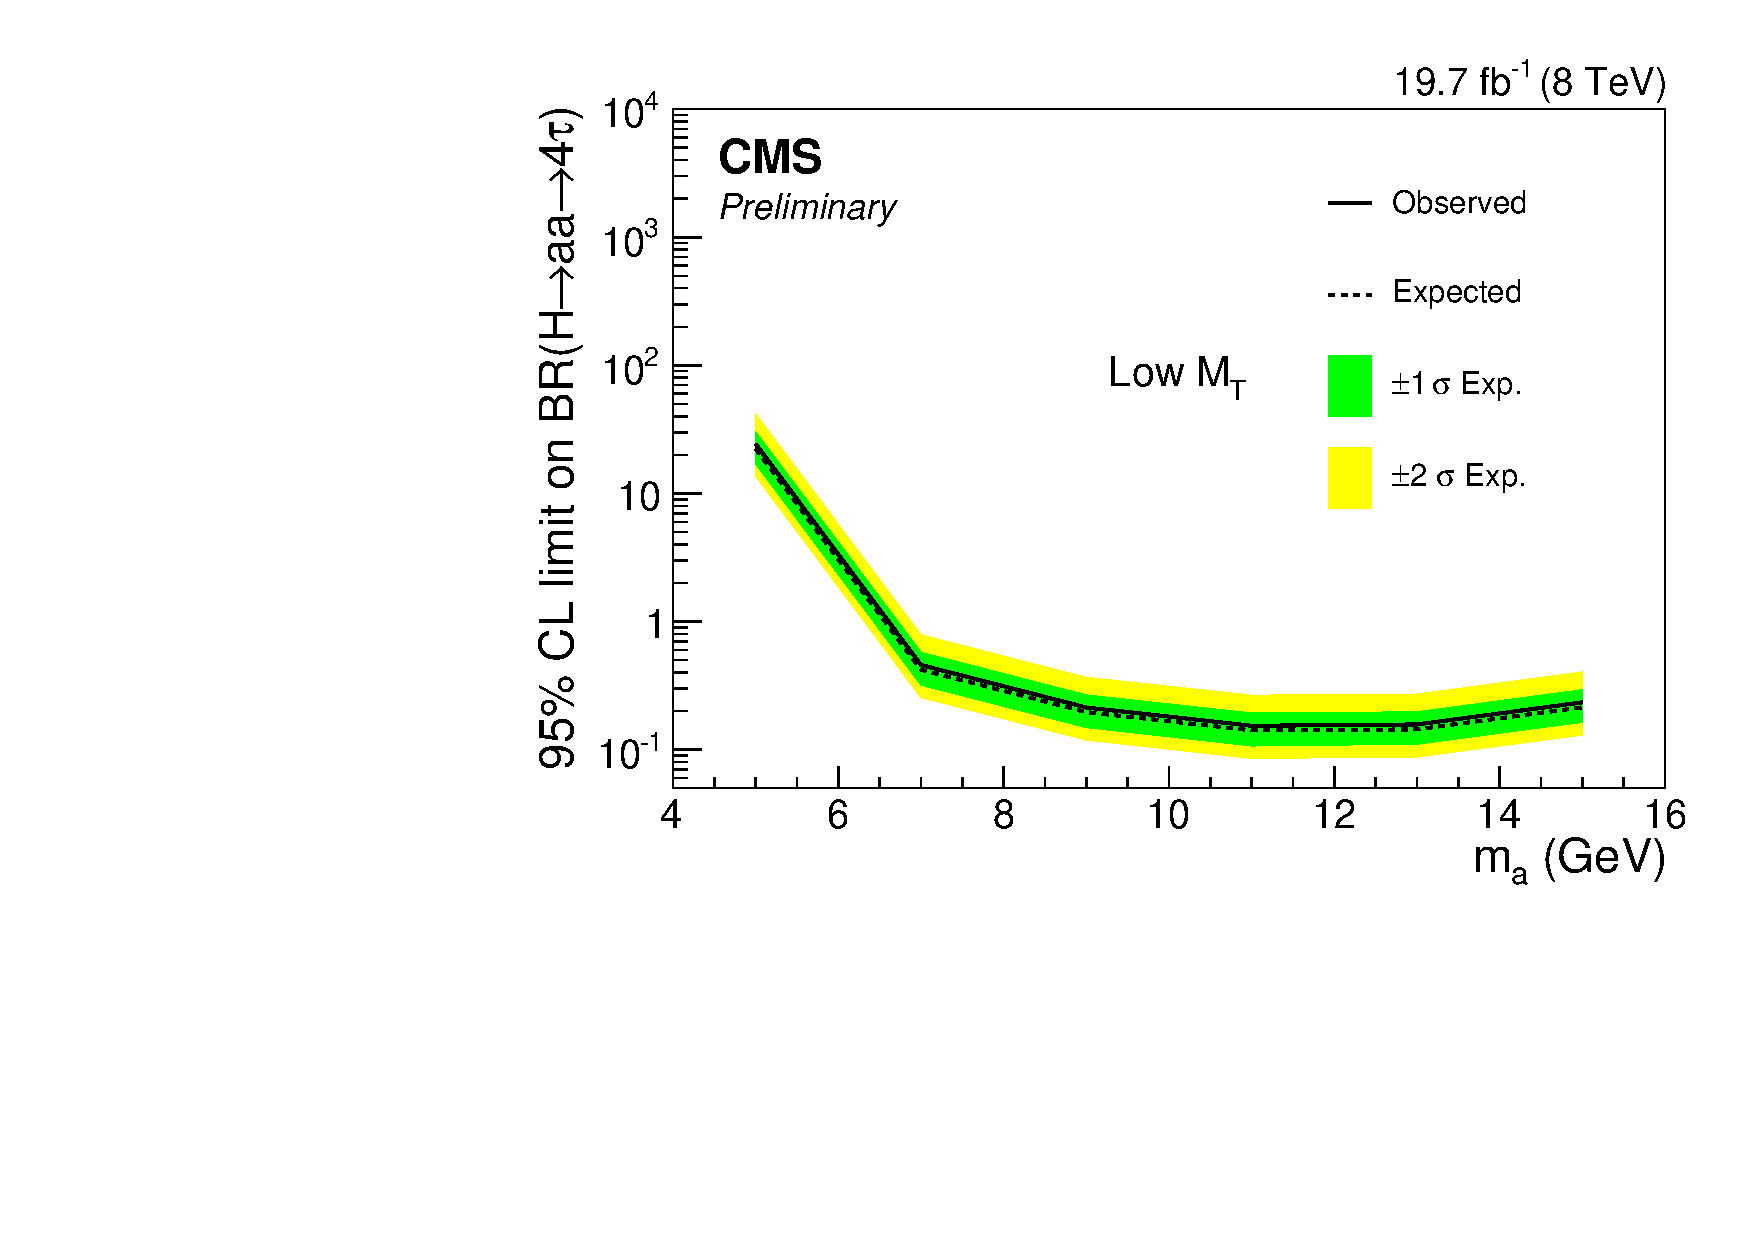
\includegraphics[width=\cmsFigWidth]{figures/expLimits_Br_lowMT_20GeV_ggHVBF}
    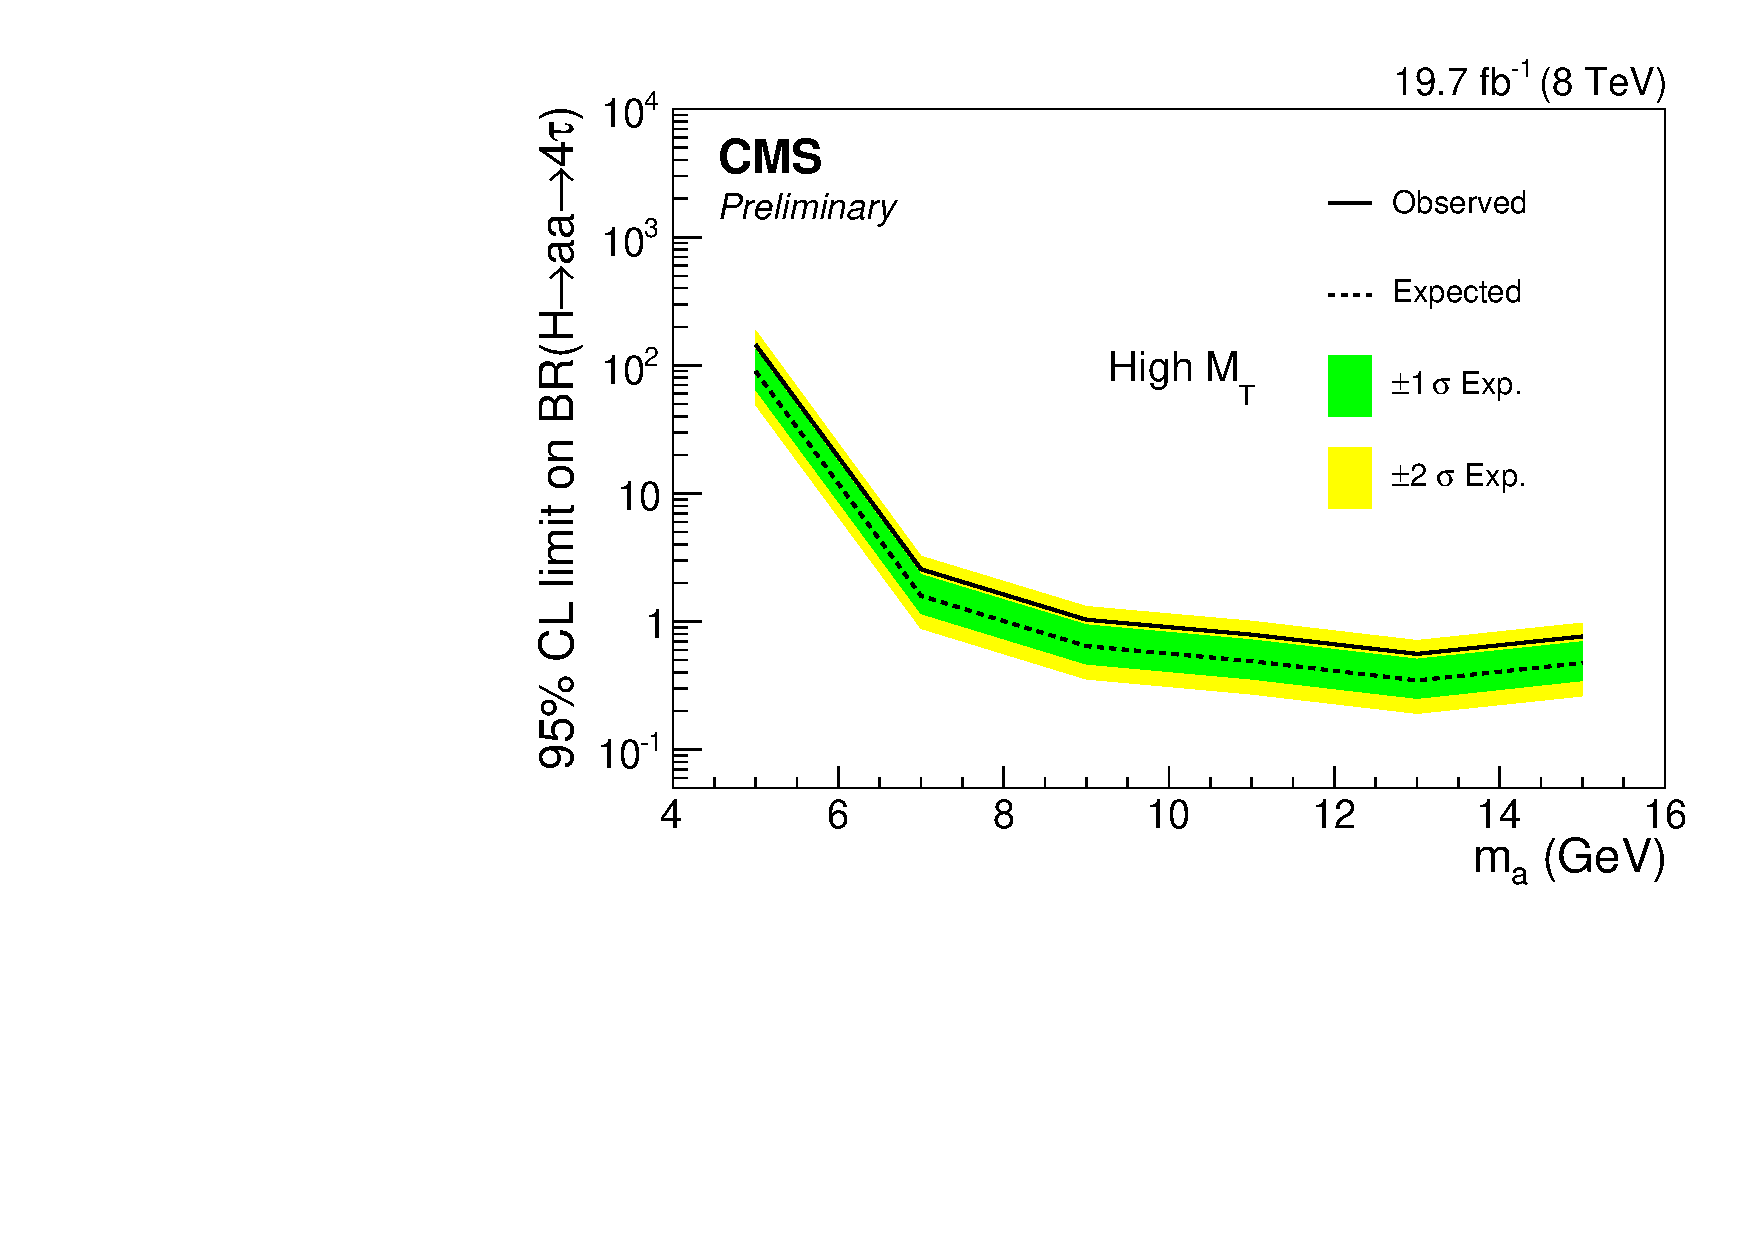
\includegraphics[width=\cmsFigWidth]{figures/expLimits_Br_highMT_20GeV_ggHWH}
    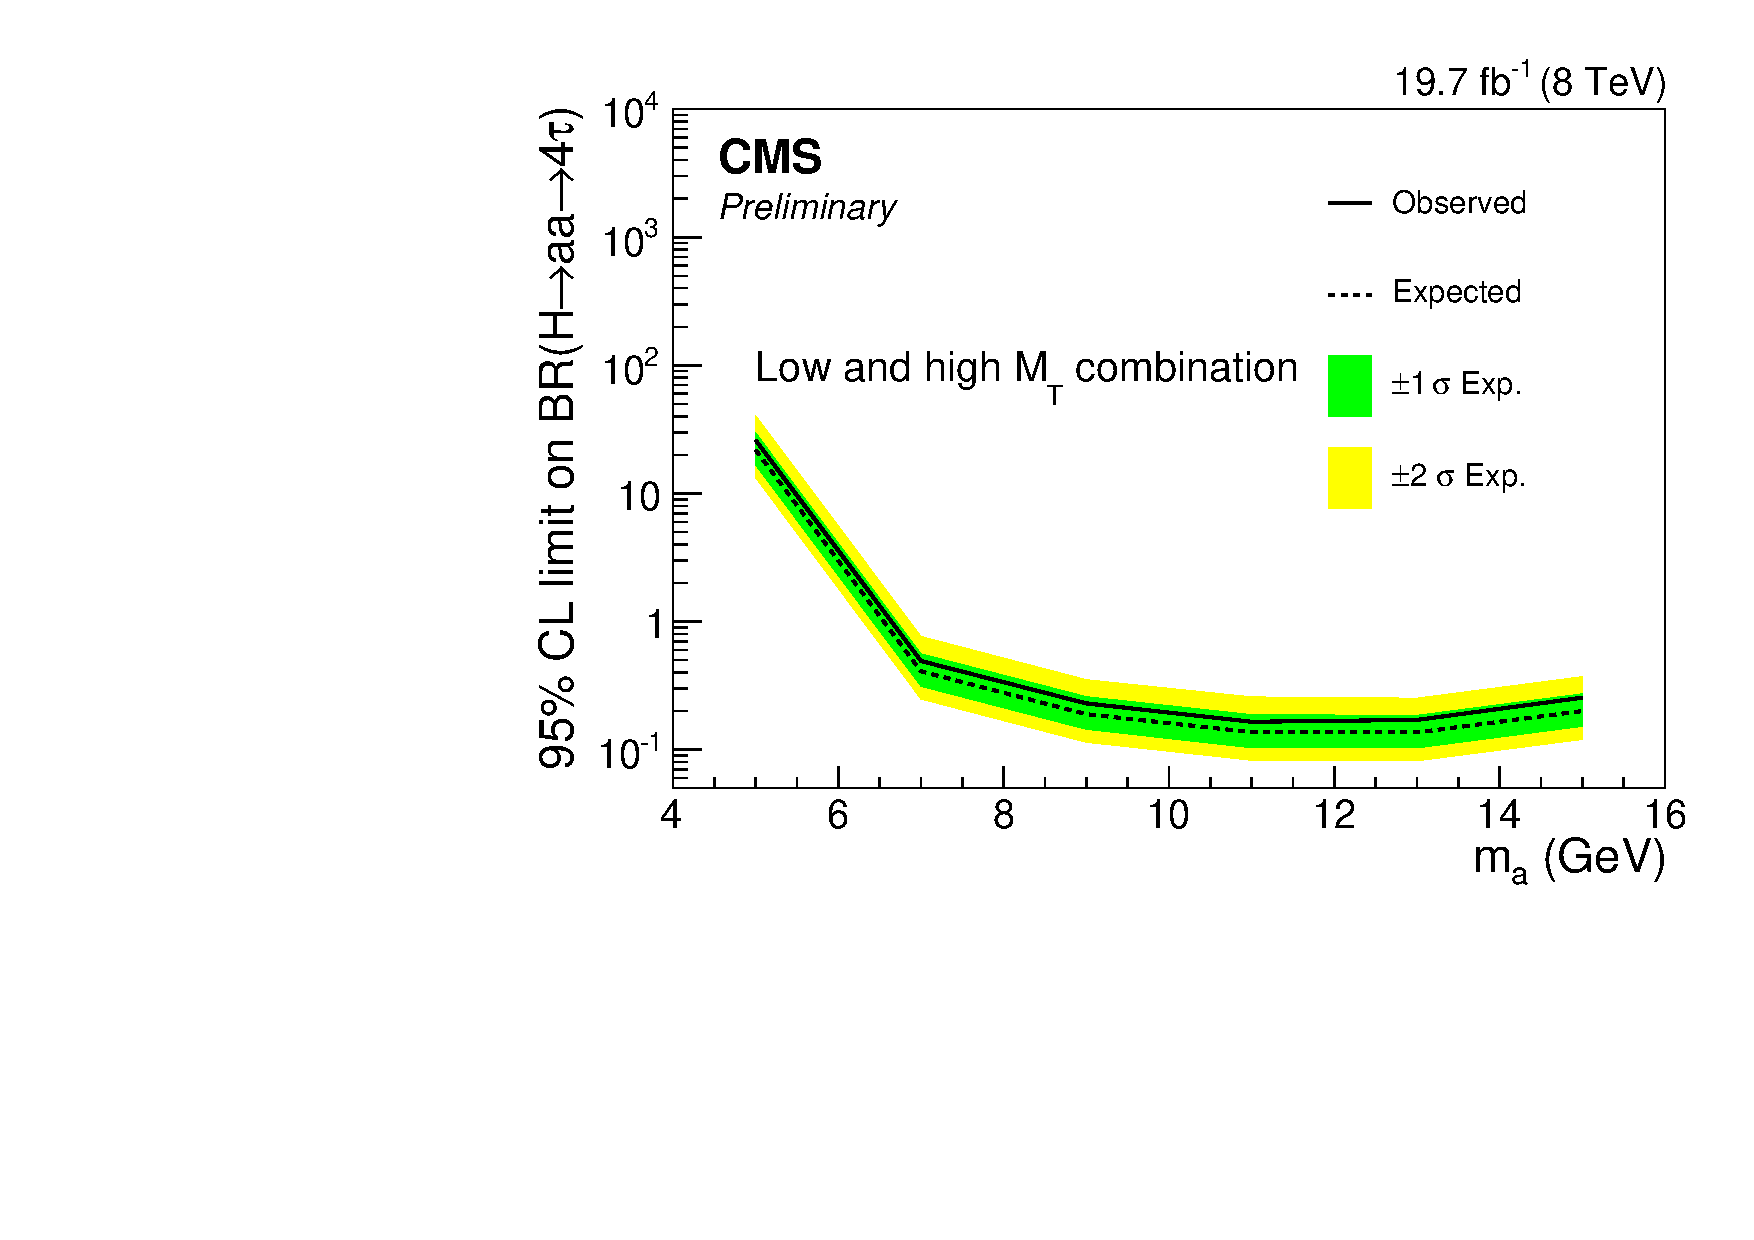
\includegraphics[width=\cmsFigWidth]{figures/expLimits_Br_20GeV_4sig}
    \caption{Observed 95\% C.L. limits (solid black curve) on the branching ratio Br($H\rightarrow$$aa\rightarrow4\tau$), compared to expected limits (dotted black curve, with $\pm1\sigma$ bands in green and $\pm2\sigma$ bands in yellow) at pseudoscalar mass points $m_{\cmsSymbolFace{a}}$ = 5 through 15 GeVcc.  (Top \cmsLeft) $M_{\text{T}}$ \textless\xspace 50 GeV. (Top \cmsRight) $M_{\text{T}}$ \textgreater\xspace 50 GeV.  (Bottom) Combined result between the low- and high-$M_{\text{T}}$ bins.}
    \label{fig:lowhighMTCLs}
  \end{center}
\end{figure}

The model-independent observed and expected $\text{CL}_{\text{S}}$ limits, expressed in terms of limits on Br($H\rightarrow$$aa\rightarrow4\tau$) assuming SM Higgs production cross-sections are tabulated in Tables~\ref{tab:CLs-limits-lowMT}-\ref{tab:CLs-limits}.

\begin{table*}
\begin{center}
  \caption{Observed and expected $\text{CL}_{\text{S}}$ limits on Br($H\rightarrow$$aa\rightarrow4\tau$) assuming SM Higgs production cross-sections in the low-$M_{\text{T}}$ bin.}
%\resizebox{\columnwidth}{!}{%
\singlespacing
\begin{tabular}{|m{3cm}|c|c|c|c|c|c|c|}
  \hline
  $m_{\cmsSymbolFace{a}}$ (GeV) & -2$\sigma$ & -1$\sigma$ & Median expected & +1$\sigma$ & +2$\sigma$ & Observed \\
  \hline
  \hline
  5 & 13.6 & 17.0 & 22.3 & 30.4 & 41.7 & 24.3 \\
  \hline
  7 & 0.255 & 0.318 & 0.420 & 0.576 & 0.787 & 0.457 \\
  \hline
  9 & 0.119 & 0.148 & 0.196 & 0.268 & 0.367 & 0.213 \\
  \hline
  11 & 0.0852 & 0.107 & 0.141 & 0.193 & 0.266 & 0.153 \\
  \hline
  13 & 0.0875 & 0.110 & 0.144 & 0.197 & 0.272 & 0.157 \\
  \hline
  15 & 0.130 & 0.163 & 0.214 & 0.294 & 0.404 & 0.234 \\
  \hline
  \end{tabular}%
%}
\label{tab:CLs-limits-lowMT}
\end{center}
\end{table*}

\begin{table*}
\begin{center}
  \caption{Observed and expected $\text{CL}_{\text{S}}$ limits on Br($H\rightarrow$$aa\rightarrow4\tau$) assuming SM Higgs production cross-sections in the high-$M_{\text{T}}$ bin.}
%\resizebox{\columnwidth}{!}{%
\singlespacing
\begin{tabular}{|m{3cm}|c|c|c|c|c|c|c|}
  \hline
  $m_{\cmsSymbolFace{a}}$ (GeV) & -2$\sigma$ & -1$\sigma$ & Median expected & +1$\sigma$ & +2$\sigma$ & Observed \\
  \hline
  \hline
  5 & 49.2 & 64.7 & 89.6 & 132 & 186 & 145 \\
  \hline
  7 & 0.883 & 1.15 & 1.59 & 2.33 & 3.23 & 2.56 \\
  \hline
  9 & 0.355 & 0.465 & 0.643 & 0.942 & 1.31 & 1.03 \\
  \hline
  11 & 0.271 & 0.355 & 0.490 & 0.719 & 1.005 & 0.789 \\
  \hline
  13 & 0.192 & 0.251 & 0.347 & 0.508 & 0.711 & 0.559 \\
  \hline
  15 & 0.262 & 0.345 & 0.475 & 0.696 & 0.973 & 0.765 \\
  \hline
  \end{tabular}%
%}
\label{tab:CLs-limits-highMT}
\end{center}
\end{table*}

\begin{table*}
\begin{center}
  \caption{Observed and expected $\text{CL}_{\text{S}}$ limits on Br($H\rightarrow$$aa\rightarrow4\tau$) assuming SM Higgs production cross-sections for the combination of the low- and high-$M_{\text{T}}$ bins.}
%\resizebox{\columnwidth}{!}{%
\singlespacing
\begin{tabular}{|m{3cm}|c|c|c|c|c|c|c|}
  \hline
  $m_{\cmsSymbolFace{a}}$ (GeV) & -2$\sigma$ & -1$\sigma$ & Median expected & +1$\sigma$ & +2$\sigma$ & Observed \\
  \hline
  \hline
  5 & 13.2 & 16.7 & 21.8 & 29.7 & 40.4 & 26.0 \\
  \hline
  7 & 0.248 & 0.312 & 0.408 & 0.560 & 0.765 & 0.491 \\
  \hline
  9 & 0.114 & 0.144 & 0.189 & 0.259 & 0.352 & 0.230 \\
  \hline
  11 & 0.0825 & 0.103 & 0.137 & 0.187 & 0.258 & 0.165 \\
  \hline
  13 & 0.0817 & 0.103 & 0.136 & 0.185 & 0.252 & 0.171 \\
  \hline
  15 & 0.120 & 0.152 & 0.200 & 0.273 & 0.371 & 0.254 \\
  \hline
  \end{tabular}%
%}
\label{tab:CLs-limits}
\end{center}
\end{table*}